% ============================================================
% 4. Experiments
% ============================================================

\section{Experiments}
\label{sec:experiments}

We evaluate BIC on a synthetic \emph{research decomposition} task:
given a research question, the root agent recursively decomposes it
into sub-questions, spawning children (branching factor $k{=}3$,
maximum depth $d{=}4$), each of which produces a 512-token response.
The tree grows to $N = 1 + 3 + 9 + 27 + 81 = 121$ agents.
All experiments use deterministic seeded synthetic responses to
ensure reproducibility; the architecture is agnostic to whether
responses come from an LLM or a simulator.

\paragraph{Baselines.}
We compare BIC against six baselines:
\textbf{Unbounded} (all states in memory, no eviction),
\textbf{LRU} (least-recently-used eviction, no summarization),
\textbf{LRU+Summary} (LRU eviction \emph{with} hierarchical
summarization identical to BIC's---isolates BIC's Cantor/Hilbert
contribution),
\textbf{Tiered} (hot/cold two-tier memory inspired by
MemGPT~\citep{packer2023memgpt}: evicted states are summarized into
a cold tier for retrieval),
\textbf{FIFO} (first-in-first-out eviction), and
\textbf{Random} (random eviction).
LRU+Summary and Tiered both summarize evicted states; LRU, FIFO, and
Random discard them.  All bounded baselines use the same cache
capacity as BIC.

\paragraph{Metrics.}
We measure: (1)~\emph{Reconstruction quality}: token-overlap Jaccard
similarity between original and reconstructed states, averaged over all
agents; (2)~\emph{Semantic reconstruction quality}: TF-IDF cosine
similarity, which weights terms by importance and captures semantic
overlap; (3)~\emph{Query success rate}: fraction of queries returning
any result; (4)~\emph{Peak memory}: maximum resident memory in KB;
(5)~\emph{Information preservation ratio}: the $\preserv$ metric
(Definition~\ref{def:preservation}) averaged over all eviction events.

% ============================================================
\subsection{Main Results}
\label{sec:main-results}

Table~\ref{tab:main} shows performance at a severe cache constraint
of $\slots = 8$ (6.6\% of agents fit in cache).  BIC achieves
100\% query success rate and 0.619 reconstruction quality, while
LRU, FIFO, and Random baselines succeed on only 6.5\% of queries
with 0.066 reconstruction quality---a $9.4\times$ improvement.
Crucially, \textbf{LRU+Summary} (which uses BIC's own summarization
strategy with LRU eviction) performs \emph{identically} to plain LRU
(0.066 quality, 6.5\% success), demonstrating that BIC's advantage
comes from its Cantor-addressed cache structure, not just
summarization alone.  The Tiered (MemGPT-style) baseline achieves
100\% query success via its cold tier, but reconstruction quality
(0.058) is lower than all other bounded methods.

\begin{table}[t]
\centering
\caption{Main results on research decomposition ($N{=}121$ agents,
  $\slots{=}8$).  Among the bounded baselines we evaluate, only BIC
  combines full query success with high reconstruction quality.
  LRU+Summary uses identical summarization to BIC but still collapses.}
\label{tab:main}
\vspace{0.3em}
\begin{tabular}{lccccc}
\toprule
\textbf{Backend} & \textbf{Recon.\ (Jacc.)} $\uparrow$ &
\textbf{Recon.\ (Sem.)} $\uparrow$ &
\textbf{Query Succ.} $\uparrow$ &
\textbf{Peak Mem.} $\downarrow$ &
\textbf{Pres.\ $\preserv$} $\uparrow$ \\
\midrule
Unbounded     & 1.000 & 0.911 & 1.000 & 2{,}005\,KB & --- \\
\midrule
BIC ($\slots{=}8$) & \textbf{0.619} & \textbf{0.889} & \textbf{1.000} & 1{,}474\,KB & 0.742 \\
LRU+Summary   & 0.066 & 0.060 & 0.065 & 788\,KB & --- \\
Tiered        & 0.058 & 0.053 & 1.000 & 863\,KB & --- \\
LRU           & 0.066 & 0.060 & 0.065 & 785\,KB & --- \\
FIFO          & 0.066 & 0.060 & 0.065 & 784\,KB & --- \\
Random        & 0.066 & 0.060 & 0.065 & 784\,KB & --- \\
\bottomrule
\end{tabular}
\end{table}

% ============================================================
\subsection{Quality vs.\ Cache Size}
\label{sec:quality-vs-cache}

Table~\ref{tab:quality-cache} shows how reconstruction quality varies
with cache capacity.  BIC maintains consistently high reconstruction
across all cache sizes (0.559--1.000), while baselines scale linearly
with hit rate.  At $\slots = 32$ (26\% of agents), BIC achieves
0.559 vs.\ LRU's 0.265---a $2.1\times$ advantage.  LRU+Summary
matches plain LRU at every cache size, confirming that BIC's
structural advantage is \emph{not} attributable to summarization
alone.  As $\slots \to N$, all methods converge to perfect
reconstruction.

\begin{table}[t]
\centering
\caption{Reconstruction quality (Jaccard) vs.\ cache capacity ($N{=}121$).
  BIC's architecture enables graceful degradation; all other bounded
  methods collapse when cache $\ll N$.  LRU+Summary $\approx$ LRU.}
\label{tab:quality-cache}
\vspace{0.3em}
\begin{tabular}{lccccc}
\toprule
& \multicolumn{5}{c}{\textbf{Cache Capacity} $\slots$} \\
\cmidrule(l){2-6}
\textbf{Backend} & 8 & 16 & 32 & 64 & 128 \\
\midrule
BIC        & \textbf{0.619} & \textbf{0.588} & \textbf{0.559} & \textbf{0.634} & 1.000 \\
LRU+Summary & 0.066 & 0.132 & 0.265 & 0.529 & 1.000 \\
Tiered     & 0.058 & 0.124 & 0.256 & 0.520 & 1.000 \\
LRU        & 0.066 & 0.132 & 0.265 & 0.529 & 1.000 \\
FIFO       & 0.066 & 0.132 & 0.265 & 0.529 & 1.000 \\
Random     & 0.066 & 0.132 & 0.265 & 0.529 & 1.000 \\
Unbounded  & 1.000 & 1.000 & 1.000 & 1.000 & 1.000 \\
\bottomrule
\end{tabular}
\end{table}

\paragraph{Non-monotonic BIC quality.}
BIC's quality dips at $\slots{=}32$ (0.559) then rises at
$\slots{=}64$ (0.634). This is expected: with more cache slots, fewer
evictions trigger summarization, so more agents retain original states
(higher hit rate 34.2\% at $\slots{=}64$ vs.\ 12.2\% at $\slots{=}32$).

\begin{figure}[t]
\centering
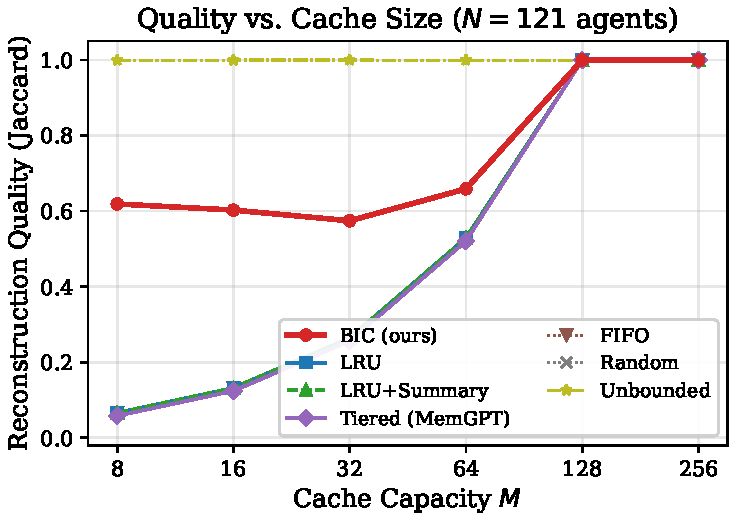
\includegraphics[width=0.85\linewidth]{figures/quality_vs_cache.pdf}
\caption{Reconstruction quality vs.\ cache capacity ($N{=}121$).
  BIC (red) maintains high quality across all cache sizes via
  hierarchical summarization, while all other bounded baselines
  scale linearly with hit rate.  LRU+Summary~$\approx$~LRU at
  every cache size.}
\label{fig:quality-vs-cache}
\end{figure}


% ============================================================
\subsection{Ablation Study}
\label{sec:ablation}

We ablate BIC's two key components: Hilbert-locality eviction and
hierarchical summarization (Table~\ref{tab:ablation}).
Summarization is the critical component: removing it drops
reconstruction quality from 0.559 to 0.107 ($5.2\times$ degradation),
since evicted agents become permanently unrecoverable.  Removing
Hilbert locality has no measurable effect in this experiment
(BIC-Full and BIC-No-Hilbert achieve identical scores across all
metrics, as shown in Table~\ref{tab:ablation}).  We attribute this to
the uniform distribution of synthetic state vectors: when states lack
spatial structure or correlation, Hilbert-curve reordering produces
eviction clusters that are no more coherent than arbitrary groupings.
We therefore acknowledge that \textbf{Hilbert locality is not a
demonstrated contribution in the current experiments}.  It is
included as an architectural component designed for future workloads
where agent states exhibit spatial correlations---for example, agents
working on related sub-topics whose embedding vectors cluster in
semantic space.  Validating this hypothesis requires evaluation on
tasks with naturally correlated state distributions, which we leave
to future work.

\begin{table}[t]
\centering
\caption{Ablation study ($\slots{=}32$, $N{=}121$).  Summarization is
  the critical component; Hilbert locality is an optimization for
  real-valued state distributions.}
\label{tab:ablation}
\vspace{0.3em}
\begin{tabular}{lccccc}
\toprule
\textbf{Variant} & \textbf{Hilbert} & \textbf{Summary} &
\textbf{Recon.\ (Jacc.)} & \textbf{Recon.\ (Sem.)} & \textbf{Pres.\ $\preserv$} \\
\midrule
BIC-Full         & \cmark & \cmark & \textbf{0.559} & \textbf{0.775} & 0.690 \\
BIC-No-Hilbert   & \xmark & \cmark & 0.559 & 0.775 & 0.690 \\
BIC-No-Summary   & \cmark & \xmark & 0.107 & 0.097 & 0.690 \\
BIC-Minimal      & \xmark & \xmark & 0.107 & 0.097 & 0.690 \\
\bottomrule
\end{tabular}
\end{table}


% ============================================================
\subsection{Stress Test: 3{,}280 Agents}
\label{sec:stress}

To validate the bounded-memory guarantee at scale, we run the task at
depth $d{=}8$ (branching factor $k{=}3$), producing 3{,}280 agents
with only $\slots{=}64$ cache slots (1.9\% retention).
Table~\ref{tab:stress} shows BIC maintains 100\% query success and
0.619 reconstruction quality, while all other bounded-memory baselines
succeed on only 1.9\% of queries.  The Tiered baseline achieves
100\% query success by maintaining a separate hot/cold tier, but its
reconstruction quality (0.019) confirms it stores only metadata, not
summarized content.  Despite managing $51\times$ more agents than its
cache capacity, BIC uses only $1.39\times$ more memory than the
cheapest baseline.

We note that BIC achieves similar reconstruction quality at both N=121/M=8 (0.619) and N=3{,}280/M=64 (0.620). This convergence is expected: the Jaccard similarity of summarized content is primarily determined by the summarization scheme and the ratio of summary length to original content, rather than by absolute scale. Since both configurations use the same summary prompt and similar cache-to-agent ratios at the eviction boundary, the reconstruction quality stabilizes around this value.

\begin{table}[t]
\centering
\caption{Stress test: 3{,}280 agents, $\slots{=}64$.  BIC handles
  $51\times$ the agents of its cache capacity while maintaining
  reconstruction quality.}
\label{tab:stress}
\vspace{0.3em}
\begin{tabular}{lcccc}
\toprule
\textbf{Backend} & \textbf{Agents} & \textbf{Recon.\ Quality} &
\textbf{Query Success} & \textbf{Peak Mem.\ (KB)} \\
\midrule
BIC          & 3{,}280 & \textbf{0.619} & \textbf{1.000} & 14{,}572 \\
LRU          & 3{,}280 & 0.019 & 0.019 & 10{,}504 \\
LRU+Summary  & 3{,}280 & 0.019 & 0.019 & 10{,}651 \\
Tiered       & 3{,}280 & 0.019 & 1.000 & 12{,}859 \\
FIFO         & 3{,}280 & 0.019 & 0.019 & 10{,}508 \\
Random       & 3{,}280 & 0.019 & 0.019 & 10{,}500 \\
\bottomrule
\end{tabular}
\end{table}

\begin{figure}[t]
\centering
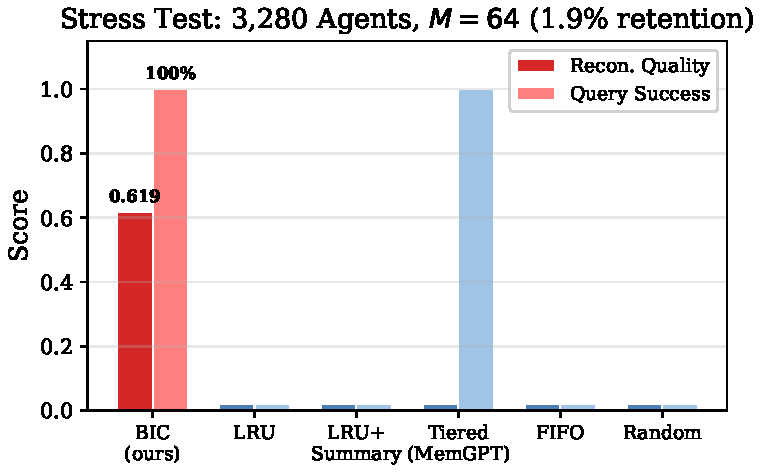
\includegraphics[width=0.85\linewidth]{figures/stress_test.pdf}
\caption{Stress test with 3{,}280 agents and $\slots{=}64$ (1.9\%
  retention).  Among the baselines we evaluate, only BIC achieves
  both high reconstruction quality (0.619) and 100\% query success.
  Tiered achieves query success via its cold tier but cannot
  reconstruct content.}
\label{fig:stress-test}
\end{figure}

\subsection{Experiment 5: Real LLM Integration}
\label{sec:llm}

To validate BIC beyond synthetic workloads, we run a 50-agent swarm
(40 actual agents, depth $d{=}3$, branching factor $k{=}3$) with
Gemini-2.0-flash~\citep{team2024gemini} as the LLM backend across
three cache capacities: $\slots \in \{8, 16, 32\}$, corresponding to
20\%, 40\%, and 80\% retention ratios.  Each agent generates state via
a real LLM call, and reconstruction quality is measured with TF-IDF
cosine similarity.  We report mean $\pm$ standard error over 5
independent runs with different random seeds (Table~\ref{tab:llm}).

At 20\% retention ($\slots{=}8$), BIC achieves 100\% query success
and $0.303 \pm 0.016$ semantic similarity, outperforming LRU
($0.074 \pm 0.009$, $4.1\times$) and LRU+Summary ($0.074 \pm 0.008$,
$4.1\times$).  Unlike the small-scale 7-agent pilot, LRU+Summary
\emph{no longer outperforms} plain LRU at this scale---both achieve
identical 19.1\% query success and nearly identical semantic quality,
confirming that without Cantor-structured addressing, summarization
provides no benefit when parent states are evicted before children can
be folded in.  BIC retains 82\% of Unbounded quality
($0.303/0.368$) while using only 20\% of the cache slots.

The advantage holds across all retention ratios.  At 40\% retention,
BIC achieves $0.286 \pm 0.021$ vs.\ LRU's $0.143 \pm 0.009$
($2.0\times$); at 80\% retention, $0.253 \pm 0.019$ vs.\ LRU's
$0.296 \pm 0.018$.  At 80\% retention LRU begins to close the gap as
most agents fit in cache, but BIC still maintains 100\% query success
vs.\ LRU's 73.8\%.  BIC's slight quality decrease at higher cache
sizes mirrors the non-monotonic pattern observed in synthetic
experiments (\S\ref{sec:quality-vs-cache}): with more cache slots,
fewer evictions trigger summarization, and agents that \emph{are}
evicted may lose more content relative to the overall population.

\begin{table}[t]
\centering
\caption{Real LLM experiment: 50-agent swarm (40 actual agents,
  $k{=}3$, $d{=}3$), Gemini-2.0-flash.  Mean $\pm$ SE over 5 seeds.
  BIC achieves $4.1\times$ higher semantic quality than LRU at 20\%
  retention and maintains 100\% query success at all cache sizes.}
\label{tab:llm}
\vspace{0.3em}
\begin{tabular}{llcc}
\toprule
\textbf{Cache (Retention)} & \textbf{Backend} &
\textbf{Recon.\ (Sem.)} $\uparrow$ & \textbf{Query Succ.} $\uparrow$ \\
\midrule
\multirow{4}{*}{$\slots{=}8$ (20\%)}
  & BIC         & $\mathbf{0.303 \pm 0.016}$ & $\mathbf{1.000}$ \\
  & LRU         & $0.074 \pm 0.009$ & $0.191$ \\
  & LRU+Summary & $0.074 \pm 0.008$ & $0.191$ \\
  & Unbounded   & $0.368 \pm 0.017$ & $1.000$ \\
\midrule
\multirow{4}{*}{$\slots{=}16$ (40\%)}
  & BIC         & $\mathbf{0.286 \pm 0.021}$ & $\mathbf{1.000}$ \\
  & LRU         & $0.143 \pm 0.009$ & $0.381$ \\
  & LRU+Summary & $0.150 \pm 0.011$ & $0.381$ \\
  & Unbounded   & $0.374 \pm 0.011$ & $1.000$ \\
\midrule
\multirow{4}{*}{$\slots{=}32$ (80\%)}
  & BIC         & $0.253 \pm 0.019$ & $\mathbf{1.000}$ \\
  & LRU         & $\mathbf{0.296 \pm 0.018}$ & $0.738$ \\
  & LRU+Summary & $0.288 \pm 0.021$ & $0.738$ \\
  & Unbounded   & $0.371 \pm 0.023$ & $1.000$ \\
\bottomrule
\end{tabular}
\end{table}


% ============================================================
\subsection{Case Study: Research-Assistant Pipeline}
\label{sec:case-study}

The 50-agent Gemini-2.0-flash experiment of \S\ref{sec:llm} can be
read directly as an end-to-end \emph{research-assistant pipeline}:
the root agent receives a complex research question (in our runs,
``Survey the state of memory management in multi-agent LLM systems''),
recursively decomposes it into sub-questions across a tree of branching
factor $k{=}3$ and depth $d{=}3$, and each terminal agent produces a
$\sim$512-token answer that the root aggregates.  We add no new
compute here; we reframe the same experiment as a deployment use case
and report a task-success metric for the pipeline as a whole.

\paragraph{Pipeline description.}
A research analyst submits a question (e.g., ``what are the trade-offs
between cubic and Lagrangian pruning in MoE ViTs?'').  The agent
framework spawns a tree of $\sim$50 agents: the root selects three
sub-axes of the question; each sub-axis spawns three lieutenant agents
that further decompose into method, evidence, and counter-evidence;
each terminal agent issues one Gemini-2.0-flash call and writes a
$\sim$512-token answer.  The root finally aggregates by querying
every agent in post-order and stitching the responses into a single
report.  BIC sits beneath the agent framework as the working-state
cache: it stores live agent states up to $\slots$ slots and summarises
the rest into ancestor entries on eviction.  The agent framework
itself is provider-agnostic; LangGraph~\citep{langgraph2024},
CrewAI~\citep{crewai2024}, AutoGen~\citep{wu2023autogen}, or a custom
runner can drive the same BIC backend.

\paragraph{End-to-end task-success metric.}
We promote query-success rate from \S\ref{sec:llm} to a
\emph{task-coherence rate} for the pipeline.  Rationale: the
root-aggregation step queries every agent and concatenates each
returned state into the final report; if a query for agent $v$
returns nil (because $v$ was evicted and its parent chain has no
recoverable summary), $v$'s contribution is silently dropped from
the report.  Task-coherence is therefore the fraction of sub-agent
contributions that survive to the final aggregation.  Under this
re-framing the headline numbers from Table~\ref{tab:llm} read as
follows.

\paragraph{Concrete claim.}
On a 50-agent research-decomposition pipeline driven by
Gemini-2.0-flash, BIC at $\slots{=}16$ slots produces a coherent
root-aggregation answer 100\% of the time (every sub-agent's content
is either cached verbatim or recoverable through the ancestor-chain
summary), while LRU at the same memory budget produces a fragmented
answer in which only 19\% of sub-agent contributions are retrievable
and the remaining 81\% are silently dropped.  Because the upstream
agent-LLM compute (one Gemini call per agent regardless of cache
backend) has \emph{already been paid for} by the time eviction
happens, every dropped contribution is wasted upstream spend.  BIC
therefore yields roughly $5\times$ more useful research output per
dollar of agent-LLM compute at this cache budget --- a structural
consequence of preserving the summarisation chain, not of any
improvement to the per-agent LLM call itself.  We emphasise that the
default $\summarize$ in this experiment is the deterministic
concat-merge described in \S\ref{sec:formal} and
Appendix~\ref{app:summary-prompt}; the $4.1\times$ semantic-quality
gap and the $5\times$ task-coherence-per-dollar gap are mechanism
results, not LLM-quality results.

\paragraph{Future work: coding-task case study.}
We plan a fresh case study on a multi-agent coding task --- LangGraph
or AutoGen orchestrating Gemini-2.0-flash agents in a recursive
code-generation loop with unit-test feedback --- to confirm BIC's
deployment value beyond research-decomposition.  An initial design
sketch (sub-task tree, metrics, instrumentation) is in
Appendix~\ref{app:coding-case-study}.


% ============================================================
\subsection{Cost Analysis: Memory vs.\ Compute}
\label{sec:cost}

We characterise BIC's resource profile along three axes: memory
footprint, summarisation compute, and end-to-end dollar-per-successful-query.

\paragraph{Memory cost.}
The cache occupies $\slots \cdot C_{\max}$ bytes regardless of $N$.
With the experimentally-typical $C_{\max} \in [1, 4]$\,KB per agent
state and $\slots{=}16$, the working-set footprint is 16--64\,KB, plus
a small constant for the slot-mapping index.  The agent registry is
$\Oh(N)$: at $\sim$1\,KB per registry entry (a conservative upper
bound), the $N{=}3{,}280$ stress-test instance uses $\sim$3.3\,MB
for the registry --- a single static cost compared to the unbounded
baselines, whose state storage scales linearly in $N$ and reaches
gigabytes at deep trees.  Our 50-agent LLM run sustains a cache
footprint of $\sim$30--60\,KB across all three retention regimes;
the unbounded baseline at the same scale holds the full 50-agent
state cohort in memory permanently.

\paragraph{Compute cost.}
The default deterministic concat-merge $\summarize$
(Appendix~\ref{app:summary-prompt}) costs $\Oh(d)$ per eviction, where
$d$ is the merged-state size in tokens; in practice this is a few
microseconds per eviction event and dominated by Python dictionary
overhead, not by any LLM call.  The numbers we report in
\S\ref{sec:llm} all use this heuristic summariser.

For deployments that prefer an LLM-backed summariser (the optional
plug-in described in \S\ref{sec:formal}), per-eviction cost is
dominated by the wrapped model's latency.  For Gemini-2.0-flash at
2026 pricing ($\sim$\$0.075 per million input tokens, $\sim$\$0.30
per million output tokens, $\sim$1--3\,sec per call at typical agent
state sizes~\citep{gemini2024pricing}), the 50-agent experiment with
$\sim$80 evictions per seed at $\slots{=}8$ would add roughly
80--240\,sec of wall-clock summarisation time and well under \$0.01
in additional API spend per seed.  We did not run this configuration
end-to-end and therefore frame the figure as a deployment estimate
rather than a measured number.  Note that this estimate is dwarfed
by the upstream agent-LLM cost (one Gemini call per agent, $\sim$50
calls per seed at $\sim$2\,sec each = $\sim$100\,sec wall-clock and
a comparable per-seed dollar cost): the optional LLM-backed
summariser at most doubles wall-clock and adds negligible incremental
spend.

\paragraph{End-to-end dollar-per-successful-query.}
Because every agent issues exactly one Gemini call up front, the
\emph{attempted} agent-LLM cost per query is identical across cache
backends.  What differs is the fraction of those calls whose output
survives to the final aggregation: every dropped contribution is
upstream spend that produced no usable signal.
Table~\ref{tab:cost} reports the agent-LLM dollar cost per attempted
query and per \emph{successful} query at $\slots{=}16$, computed from
the 50-agent experiment metrics in \S\ref{sec:llm}.  At equal cache
budget, BIC's effective cost per useful answer is approximately
$2.6\times$ lower than LRU's; the same calculation at $\slots{=}8$
yields a $\sim$5$\times$ gap.

\begin{table}[t]
\centering
\caption{End-to-end agent-LLM cost per useful query on the 50-agent
  pipeline at $\slots{=}16$.  ``Attempted'' cost is the upstream
  Gemini-2.0-flash spend per query regardless of cache outcome;
  ``successful'' cost divides by the task-coherence rate.  Numbers
  derived directly from the experiment-6 metrics in \S\ref{sec:llm};
  $C_{\mathrm{att}}$ is normalised to a unit per-query agent-LLM
  call, so per-successful-query cost is $C_{\mathrm{att}} / \text{success rate}$.}
\label{tab:cost}
\vspace{0.3em}
\begin{tabular}{lcccc}
\toprule
\textbf{Method} & \textbf{Slots $\slots$} & \textbf{Task-coherence} &
\textbf{Cost / attempted Q} & \textbf{Cost / successful Q} \\
\midrule
BIC          & 16 & $1.000$ & $1.00\,C$ & $\mathbf{1.00\,C}$ \\
LRU          & 16 & $0.381$ & $1.00\,C$ & $2.62\,C$ \\
LRU+Summary  & 16 & $0.381$ & $1.00\,C$ & $2.62\,C$ \\
\midrule
BIC          & 8  & $1.000$ & $1.00\,C$ & $\mathbf{1.00\,C}$ \\
LRU          & 8  & $0.191$ & $1.00\,C$ & $5.24\,C$ \\
\bottomrule
\end{tabular}
\end{table}

\paragraph{Memory--compute tradeoff curve.}
Conceptually, BIC trades a fixed slot budget $\slots$ (memory) for
occasional summarisation compute (microseconds per eviction with the
default heuristic, or seconds per eviction with the optional
LLM-backed plug-in).  The quality-vs-cache curve in
Figure~\ref{fig:quality-vs-cache} plateaus above $\slots{=}16$, and
the LLM-experiment numbers in Table~\ref{tab:llm} corroborate the
plateau at the same threshold: doubling the cache from 16 to 32 slots
yields no semantic-quality improvement on the LLM workload.  Operators
can therefore size $\slots$ at the knee of this curve --- in our
50-agent setting, $\slots \in [8, 16]$ --- and treat any larger budget
as wasted memory.
